\chapter{实验设计与结果分析}

\section{实验设置}

\subsection{数据划分策略}

本文设置随机样本划分和单井深度区间隔离划分两类协议。随机样本划分将样本打乱后分配到训练集和验证集，用于先导性地判断输入与标签之间是否存在可学习关系。由于测井样本沿深度连续，相邻窗口可能共享相似波形、地层和标签，随机划分会使邻近样本出现在不同集合中。结构化数据验证研究指出，此类依赖可能导致预测误差被低估\cite{Roberts2017CrossValidation,Valavi2019BlockCV,Ploton2020SpatialValidation}。因此，随机样本划分结果不用于表征最终泛化能力。

主要回归实验采用单井深度区间隔离划分。训练、验证和测试井段按深度连续分隔，并在相邻集合之间保留 5~ft 缓冲区。划分结果见表 \ref{tab:depth-split}。三个集合的深度键无交集，缓冲区内 19 个样本被排除。

\begin{table}[htbp]
  \centering
  \caption{单井深度区间隔离划分}
  \label{tab:depth-split}
  \begin{tabular}{lrrr}
    \toprule
    集合 & 样本数 & 起始深度/ft & 终止深度/ft \\
    \midrule
    训练集 & 1984 & 2732.440 & 3715.853 \\
    验证集 & 416 & 3721.119 & 3917.685 \\
    测试集 & 423 & 3922.785 & 4129.744 \\
    \bottomrule
  \end{tabular}
\end{table}

该协议检验模型从较浅连续区间迁移到更深连续区间的能力，比同井随机划分更严格，但仍属于单井验证。地层和仪器域变化仅限同一口井，不能据此推断跨井性能。

\subsection{对照实验设置}

本文使用三个正式实验名称：

\begin{enumerate}
  \item 基于 CWT 特征的窜槽二分类可学习性验证实验（以下简称实验一）；
  \item 基于一维窜槽占比标签的回归对照实验（以下简称实验二）；
  \item 基于方位旋转不变 FFT 幅值标签的窜槽结构特征反演实验（以下简称实验三）。
\end{enumerate}

实验一采用随机样本划分，只回答 CWT 输入是否含有与 CAST 派生二分类标签相关的可学习信号。实验二和实验三采用相同的单井深度区间隔离划分，分别比较一维占比标签与 $70\times30$ FFT 幅值标签。实验三是本文针对方位失配问题的主要实验。

\subsection{模型训练参数}

实验三使用第 3 接收环的 $150\times400\times8$ CWT 输入，模型输出为 $70\times30$。训练采用 Adam 优化器、初始学习率 $1\times10^{-4}$、批量大小 8、Huber 损失和 0.5 的 Dropout。最大训练轮数设为 80，早停耐心值为 10；同时根据验证损失降低学习率。数据增强包括小幅噪声和频率掩膜，最前 30 个时间采样使用伪影掩膜。训练在 NVIDIA A100 GPU 环境完成。

实验三实际训练 12 轮，验证损失在第 2 轮达到最小值 0.015220，早停后恢复第 2 轮权重。实验二使用相同的数据划分和输入处理框架，其最佳完成结果用于本章比较。

\section{随机样本划分条件下的先导实验}

随机样本划分先导实验的目的不是给出泛化结论，而是排除“XSI 时频输入与 CAST 派生标签完全无关”的可能性。实验一在随机样本划分下取得验证 AUC 0.95361、验证准确率 0.885366。该结果说明在该划分条件下，CWT 输入包含可用于区分 CAST 派生窜槽类别的统计信息。

然而，相邻深度样本并非完全独立。高 AUC 可能同时反映真实可学习关系和邻近样本相似性。按照分块验证研究的建议\cite{Roberts2017CrossValidation,Meyer2018TargetValidation}，本文只把实验一作为可学习性验证，不将其写成跨深度、跨井或工程应用性能。

\begin{table}[htbp]
  \centering
  \caption{实验一的随机样本划分验证结果}
  \label{tab:exp1}
  \begin{tabular}{lccp{0.42\textwidth}}
    \toprule
    输入与任务 & 验证 AUC & 验证准确率 & 解释边界 \\
    \midrule
    CWT 二分类 & 0.95361 & 0.885366 & 仅说明随机样本划分下存在可学习信号 \\
    \bottomrule
  \end{tabular}
\end{table}

\section{实验三整体性能}

\subsection{训练过程}

图 \ref{fig:exp3-training} 给出训练与验证损失。验证损失在第 2 轮达到最小，之后没有继续改善；训练过程持续至第 12 轮并触发早停。较早出现最佳验证点、后续训练损失继续下降而验证改善有限，表明模型存在过拟合倾向。这与样本量有限、输出维度较高和标签稀疏的条件一致，但这些因素只是可能解释，不能由损失曲线单独证明。

\begin{figure}[htbp]
  \centering
  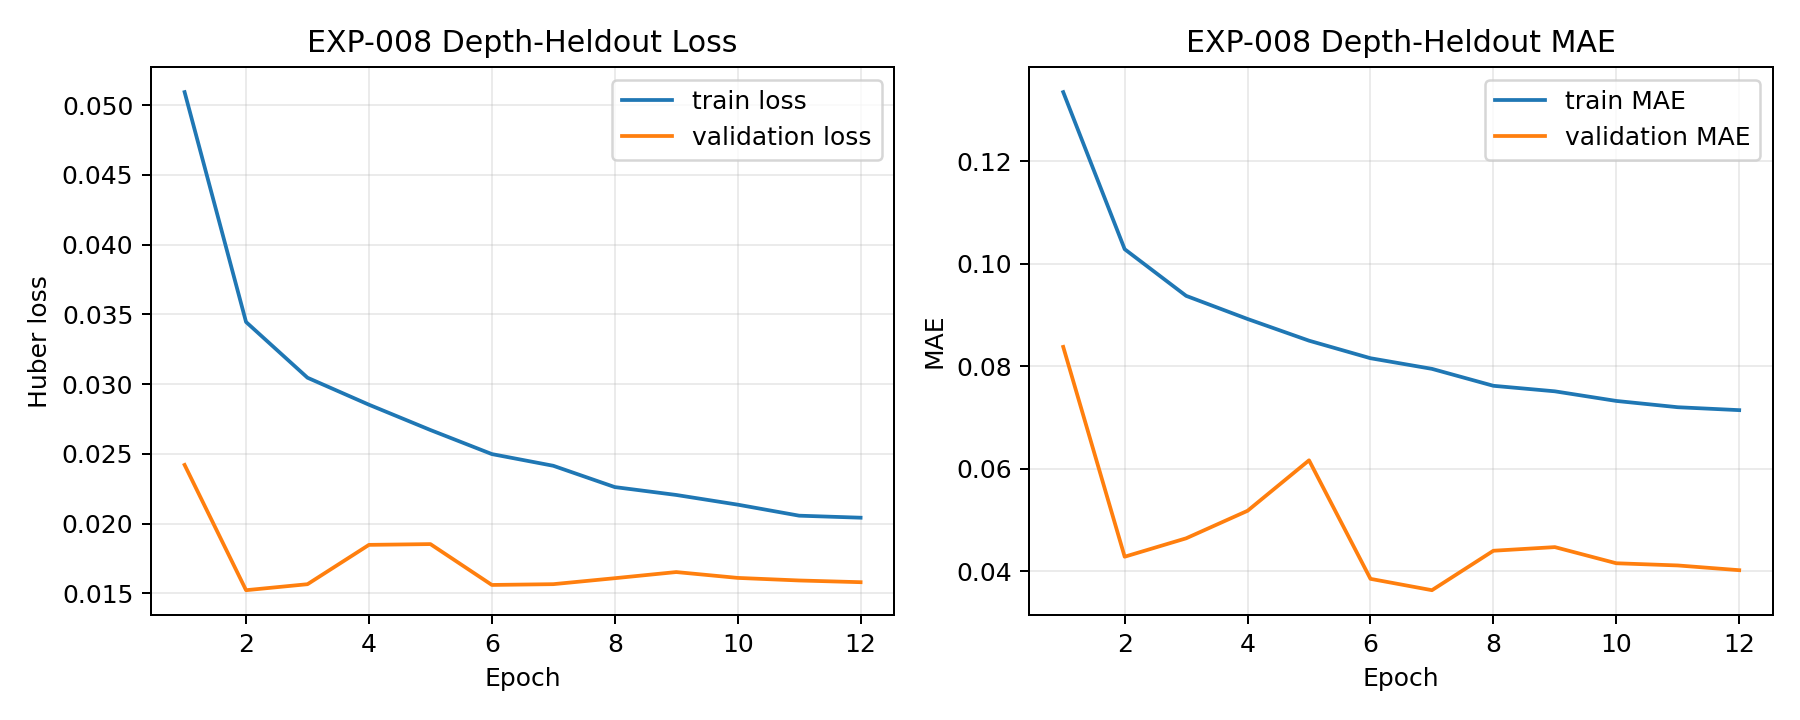
\includegraphics[width=0.94\textwidth]{figures/revision/exp3_training_curve.png}
  \caption{实验三训练损失与验证损失曲线}
  \label{fig:exp3-training}
\end{figure}

\subsection{验证集与测试集指标}

实验三的验证集和测试集指标见表 \ref{tab:exp3-metrics}。测试集包含 423 个样本、888300 个标签元素。测试 $R^2=0.106634$，说明模型相对测试标签均值只能解释有限比例的方差；Pearson 系数 0.351950、Spearman 系数 0.480519，表现为中等偏弱的正相关。该结果支持“存在一定可学习性”，不支持“高精度反演”。

\begin{table}[htbp]
  \centering
  \caption{实验三的验证集与测试集整体指标}
  \label{tab:exp3-metrics}
  \begin{tabular}{lrrrrrr}
    \toprule
    集合 & MAE & RMSE & $R^2$ & Pearson & Spearman & $n$ \\
    \midrule
    验证集 & 0.042817 & 0.187167 & 0.010882 & 0.200575 & 0.266137 & 416 \\
    测试集 & 0.079025 & 0.277019 & 0.106634 & 0.351950 & 0.480519 & 423 \\
    \bottomrule
  \end{tabular}
\end{table}

预测与真实值散点见图 \ref{fig:exp3-scatter}。大量标签元素聚集在零值附近，非零标签分布更分散。模型能够产生与真实值同向变化的响应，但对较大目标的覆盖不足；这与较低的 $R^2$ 和有限相关性相一致。

\begin{figure}[htbp]
  \centering
  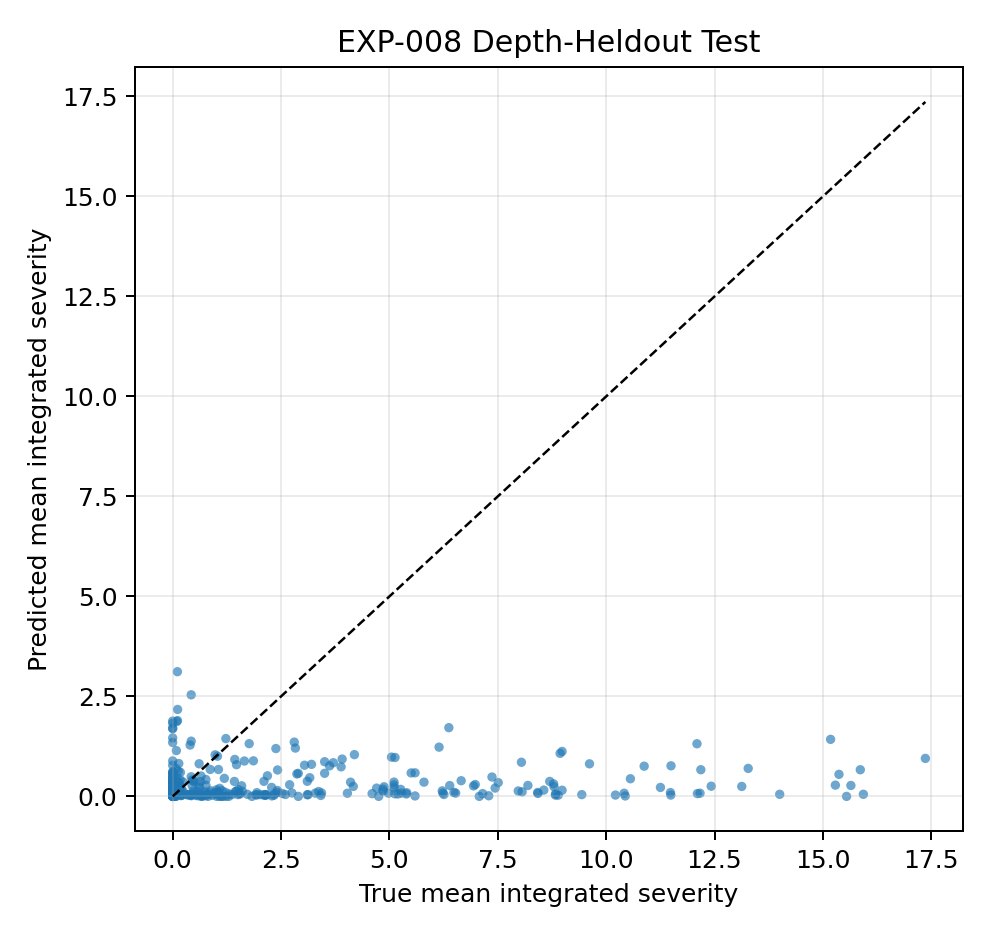
\includegraphics[width=0.72\textwidth]{figures/revision/exp3_prediction_scatter.png}
  \caption{实验三测试集预测值与真实值散点}
  \label{fig:exp3-scatter}
\end{figure}

\section{基线比较}

表 \ref{tab:exp3-baseline} 和图 \ref{fig:exp3-baseline} 比较模型与三类简单基线。零值基线将全部 $70\times30$ 标签预测为 0；训练集均值和中位数基线分别用训练标签的逐元素统计量预测测试样本。

\begin{table}[htbp]
  \centering
  \caption{实验三与简单基线的测试集比较}
  \label{tab:exp3-baseline}
  \begin{tabular}{lrrr}
    \toprule
    方法 & MAE & RMSE & $R^2$ \\
    \midrule
    本文模型 & 0.079025 & 0.277019 & 0.106634 \\
    零值基线 & \textbf{0.069751} & 0.301272 & -0.056638 \\
    训练集均值基线 & 0.142358 & 0.316129 & -0.163426 \\
    训练集中位数基线 & 0.119024 & 0.278963 & 0.094049 \\
    \bottomrule
  \end{tabular}
\end{table}

\begin{figure}[htbp]
  \centering
  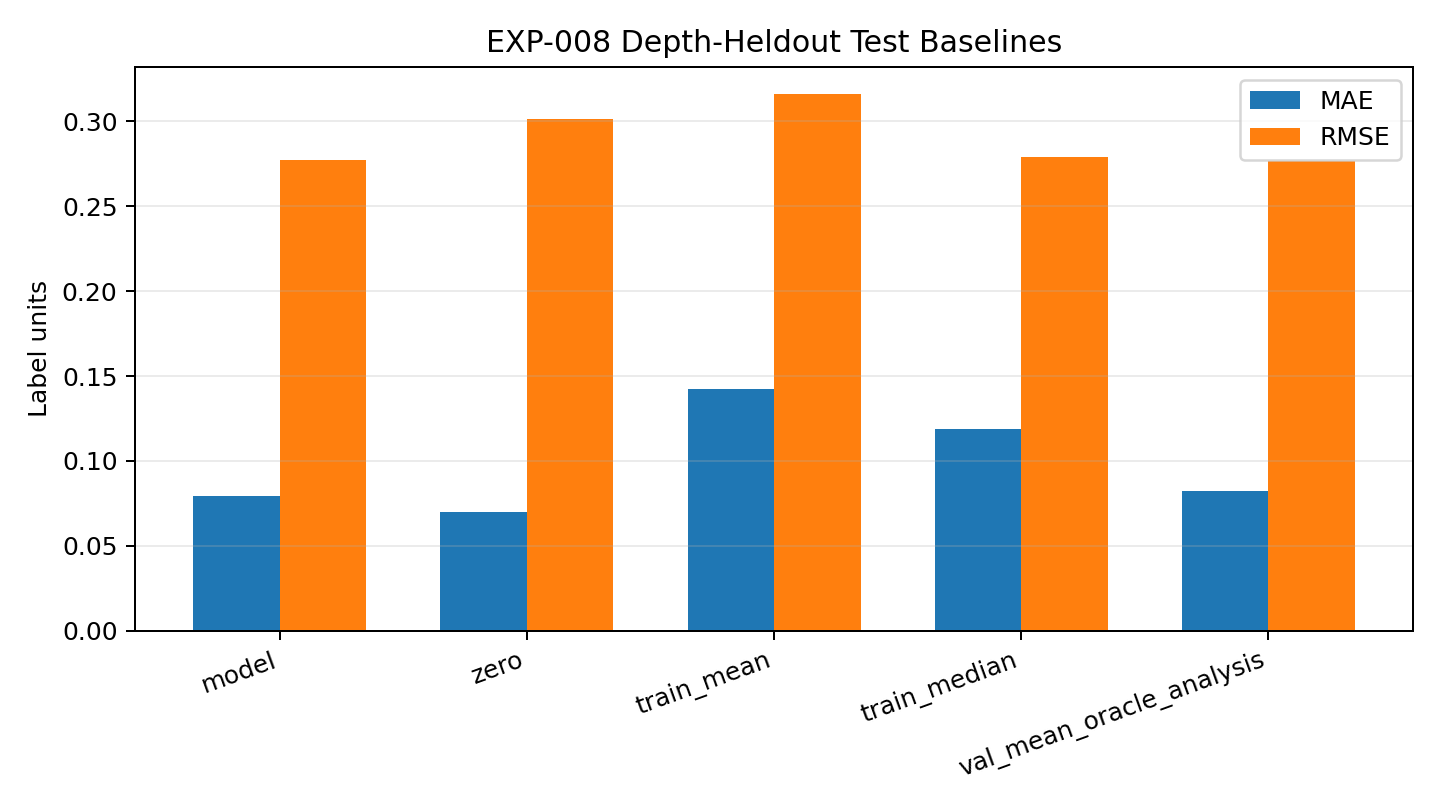
\includegraphics[width=0.91\textwidth]{figures/revision/exp3_baseline_comparison.png}
  \caption{实验三模型与简单基线的 MAE、RMSE 和 $R^2$}
  \label{fig:exp3-baseline}
\end{figure}

比较结果具有指标依赖性。模型的 MAE 没有优于零值基线，说明标签稀疏时“全部预测为零”可获得较低平均绝对误差；但模型的 RMSE 和 $R^2$ 优于零值基线，表明模型对部分非零结构的预测减少了较大平方误差。模型在三项指标上均优于训练集均值基线。与训练集中位数基线相比，模型 RMSE 只改善 0.001944，差距很小；$R^2$ 略高，MAE 较低。因而不存在“所有指标全面领先”的结论。

标签元素的绝对误差中有较高比例集中在零附近，使 MAE 对稀疏区域权重较大。RMSE 对大误差更敏感，$R^2$ 又以测试集方差为参照，三者回答的问题不同。本文保留全部指标，不选择性报告对模型有利的结果。

\section{FFT 系数误差}

图 \ref{fig:exp3-coeff} 给出 $k=0$--29 各系数 MAE。测试集中 $k=0$--4 的平均 MAE 为 0.131411；按既有汇总口径，$k=0$--5 的 MAE 为 0.128785，而 $k=15$--29 的 MAE 为 0.050184。低阶系数包括周向总量和较大尺度结构，其目标幅值总体较大，因此绝对误差也较高。

\begin{figure}[htbp]
  \centering
  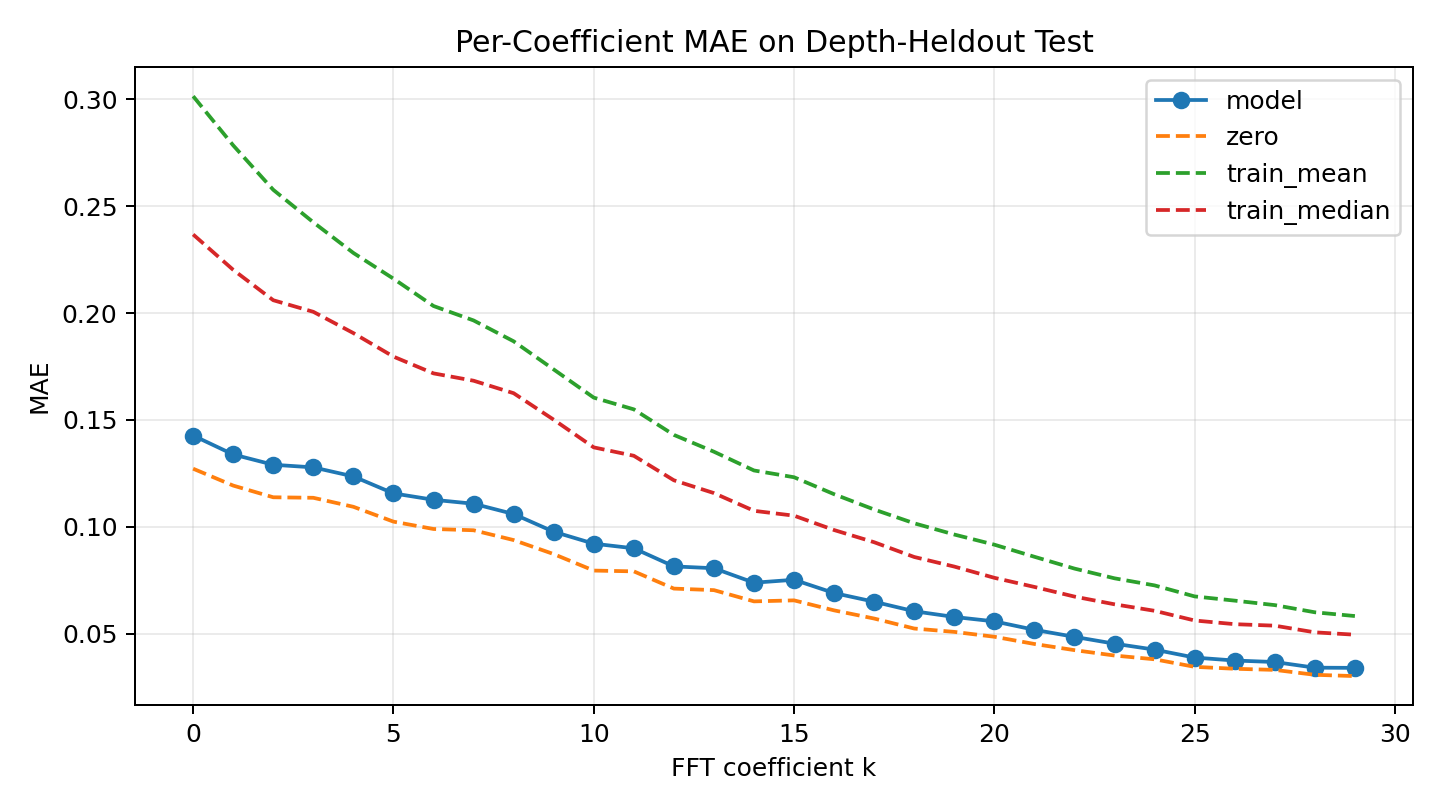
\includegraphics[width=0.93\textwidth]{figures/revision/exp3_coefficient_mae.png}
  \caption{实验三各方位 FFT 系数的测试 MAE}
  \label{fig:exp3-coeff}
\end{figure}

高阶系数 MAE 较小不能直接解释为“高频结构更容易学习”。当目标系数本身接近零时，即使模型忽略其变化，绝对误差也可能较小。因而需要结合目标幅值、归一化误差和结构重构共同判断。现有证据只支持低阶系数是总体绝对误差的重要组成部分。

\section{高严重度样本误差}

为观察标签分布，将测试样本按真实平均积分严重度分组。423 个测试样本中，177 个为零，171 个位于 $(0,5)$，75 个位于 $[5,20)$，没有样本达到 20 以上。该分布说明测试集同时具有大量零样本和有限的较高严重度样本。

图 \ref{fig:exp3-lowfreq} 比较低频摘要的真实值与预测值。误差较大的高严重度样本中，预测通常低于真实峰值，结果提示模型可能存在向样本中心收缩的倾向。可能原因包括较高严重度样本数量有限、ReLU 多输出回归的稀疏目标、损失由大量低值元素主导以及同井深度区间分布变化。现有实验没有逐项验证这些机制，因此只能将其列为可能因素。

\begin{figure}[htbp]
  \centering
  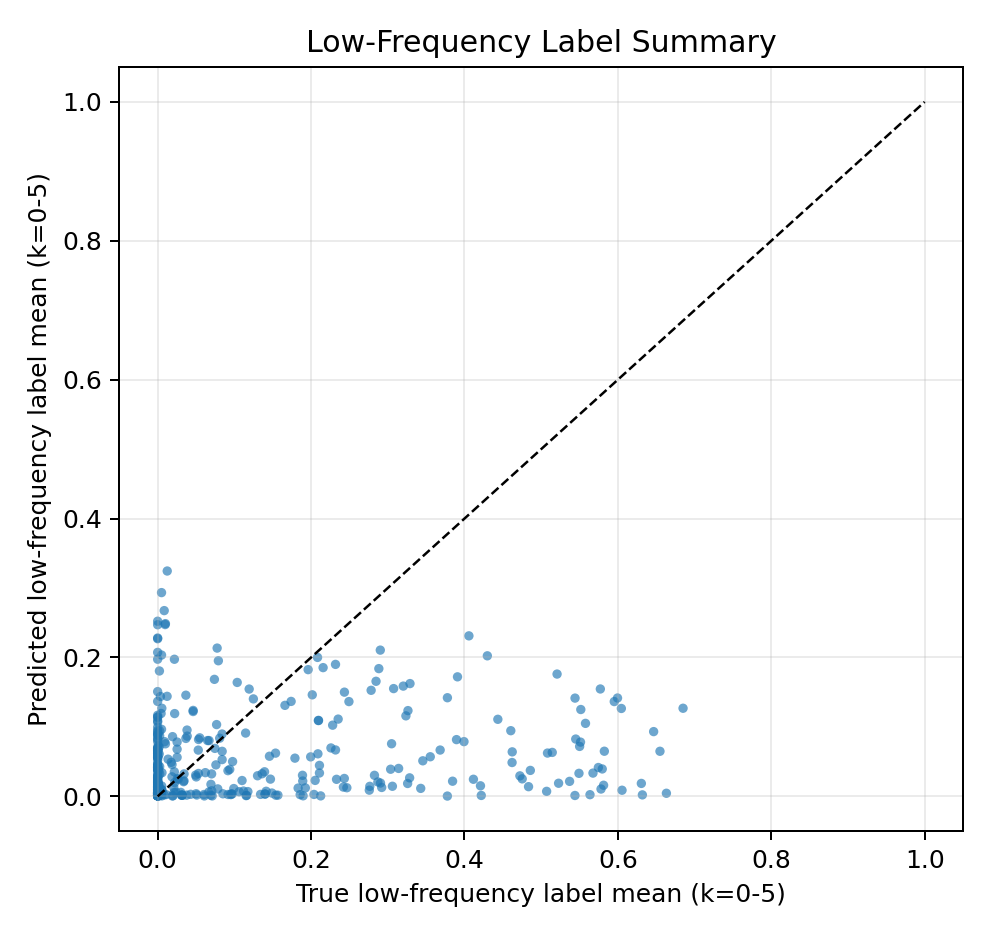
\includegraphics[width=0.72\textwidth]{figures/revision/exp3_lowfreq_summary.png}
  \caption{实验三低频结构摘要的真实值与预测值比较}
  \label{fig:exp3-lowfreq}
\end{figure}

测试残差分布见图 \ref{fig:exp3-error}。分布集中于零附近但存在长尾，与 RMSE 高于 MAE 所反映的少量较大误差一致。对固井质量研究而言，较高严重度样本更值得关注；因此，总体平均指标不能替代分组误差分析。

\begin{figure}[htbp]
  \centering
  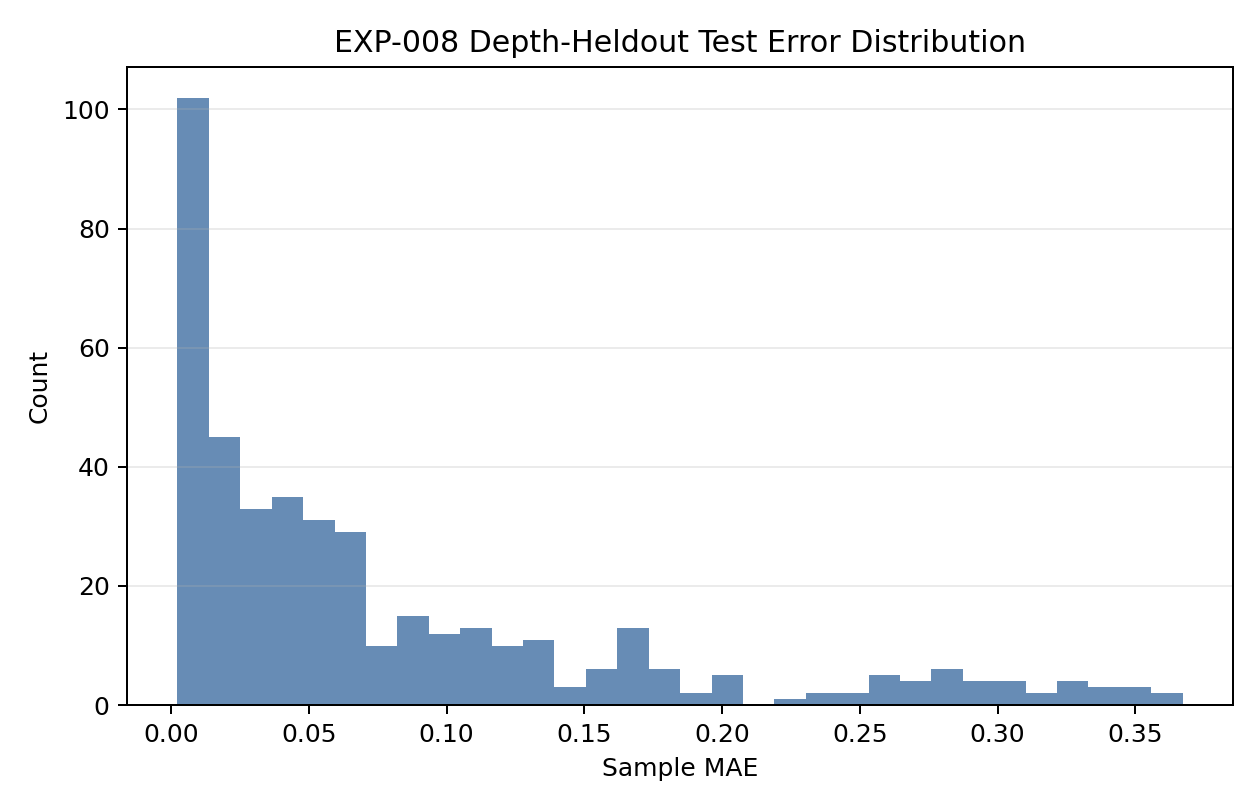
\includegraphics[width=0.88\textwidth]{figures/revision/exp3_error_distribution.png}
  \caption{实验三测试集标签元素误差分布}
  \label{fig:exp3-error}
\end{figure}

\section{实验二对照结果}

实验二使用一维窜槽占比标签，将每个深度位置的 180 个周向采样压缩为一个占比。输出维度降低后，模型不再需要预测方位结构，但仍要从 XSI 时频响应迁移到隔离测试井段。测试结果见表 \ref{tab:exp2-metrics}。

\begin{table}[htbp]
  \centering
  \caption{实验二的单井深度区间隔离测试指标}
  \label{tab:exp2-metrics}
  \begin{tabular}{lr}
    \toprule
    指标 & 数值 \\
    \midrule
    MAE & 0.811672 \\
    RMSE & 2.832056 \\
    $R^2$ & -0.011278 \\
    Pearson & 0.198048 \\
    Spearman & 0.413335 \\
    \bottomrule
  \end{tabular}
\end{table}

负 $R^2$ 表明实验二在平方误差意义下未优于以测试均值为参照的常数预测。Pearson 相关较弱，Spearman 为正，说明预测排序中仍有部分信息，但幅值拟合不足。该结果说明，简单降低标签维度并未消除深度区间迁移困难。一维标签对照的价值在于揭示方位平均造成的信息损失，而不是提供比实验三更强的性能结论。

\section{实验一结果的使用边界}

实验一的高验证 AUC 仅在随机样本划分条件下成立。与实验二、实验三的深度区间隔离结果相比，它说明 CWT 输入中存在与 CAST 派生标签相关的可学习信号，却不能回答该信号能否稳定迁移到未见连续井段。本文不把二分类准确率与回归 MAE、$R^2$ 直接比较，也不以实验一替代主实验的严格验证。

\section{Grad-CAM 可解释性分析的证据边界}

Grad-CAM 的方法定义和解释边界已在第 3 章给出\cite{Selvaraju2017GradCAM}。现有候选图件可部分追溯到早期 FFT 回归分析脚本，但无法把每张图唯一对应到生成时的模型 checkpoint、训练运行、样本深度和数据划分；分析脚本还将全部回归输出之和作为标量目标，不能据此解释某一特定深度位置或 FFT 系数。因此，这些图件不满足本文主要实验的结果准入条件，本章不插入热图，也不声称已经完成单井深度区间隔离模型的 Grad-CAM 验证。

这一取舍不影响前述预测指标和误差分析。后续只有在模型版本、划分、checkpoint、样本深度、目标输出和卷积层同时可追溯时，才适合比较不同样本的时频响应区域；即使证据链完整，热图也只能解释为针对特定预测的梯度加权特征响应，不能作为物理因果证据。

\section{本章小结}

本章在相同单井深度区间隔离划分下比较了两种回归标签，并以随机样本划分二分类作为先导验证。实验三测试 MAE 为 0.079025、RMSE 为 0.277019、$R^2$ 为 0.106634，相关性为中等偏弱，支持有限可学习性而非高精度结论。模型在 RMSE 和 $R^2$ 上优于零值基线，却未在 MAE 上占优；与训练集中位数基线的 RMSE 接近。低阶 FFT 系数和较高严重度样本构成主要误差来源。实验二降低输出维度后 $R^2$ 仍为负，说明深度区间迁移并未因标签简化而解决。来源链不完整的 Grad-CAM 图件未作为实验结果使用。
